\documentclass[aspectratio=169]{beamer}

\mode<presentation>

  \usetheme{Copenhagen}
  \setbeamercovered{transparent}
%  \usecolortheme{seahorse}
%  \usecolortheme{rose}
%  \usecolortheme{wolverine}
  \useoutertheme{infolines}


\usepackage[T1]{fontenc}
\usepackage[serbian]{babel}
\usepackage[cp1250]{inputenc}
\usepackage{times}


\usepackage{graphics}
\usepackage{eurosym}
\usepackage{multirow}
\usepackage{multimedia}
\usepackage{color}
\usepackage{multirow}
\usepackage{subfig}

\title[Simulacija zagu\v{s}enja \hspace{1em} {\scriptsize \insertframenumber\ / \inserttotalframenumber}]
{Simulacija zagu\v{s}enja pomo\'{c}u ns-3\\[3ex]
\small
projekat iz predmeta\\
Principi modernih telekomunikacija (IR3PMT)\\
2023.}

\author[A. Popovi\'{c} --- IR3PMT 2023.]{Aleksandar Popovi\'{c}}

\date[]{}


%\AtBeginSection[]
%{
%  \begin{frame}<beamer>
%    \frametitle{Sadr�aj}
%    \tableofcontents[currentsection,hideothersubsections]
%  \end{frame}
%}


%\beamerdefaultoverlayspecification{<+->}


\begin{document}

\begin{frame}
%  \vfill
  \titlepage
\end{frame}


\begin{frame}
    \frametitle{Sadr�aj}
    \tableofcontents
\end{frame}


\section{Simulator}
% nazivi odeljaka ce se prikazati u sadrzaju

\begin{frame}

\begin{columns}
	\column{.60\textwidth}
	  \begin{itemize}
		\item <1-> Simulator mre\v{z}a
		\item  <2-> Softver otvorenog koda
		\item <3-> Skripte se pi\v{s}u u jeziku C++
		% <k-> znaci da se sadrzaj u tom redu prikazuje od k-tog klika nadalje
	\end{itemize}
	\column{.40\textwidth}
	\begin{figure}[t]
		\centering
		
\includegraphics[width=\textwidth]{../slike/ns-3.png}
	\end{figure}
\end{columns}

\end{frame}

\section{Simulacija}
\subsection{Opis simulacije}
\begin{frame}
	\begin{columns}
		\column{0.5\textwidth}
		\begin{itemize}
			\item <1-> Proizvodimo zagu\v{s}enje
			\item <2-> Ra\v{c}unari 2 i 3 \v{s}alju UDP pakete ka 0
		\end{itemize}
		\column{0.5\textwidth}
		\begin{figure}
			\centering
			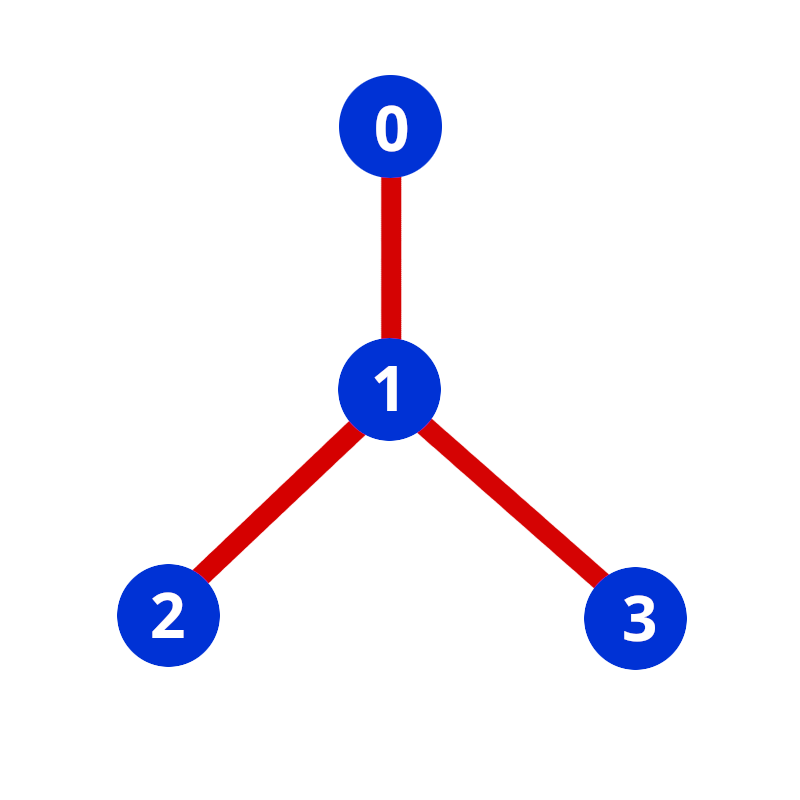
\includegraphics{../slike/topologija_simple.png}
		\end{figure}
	\end{columns}
\end{frame}

\subsection{Prvobitna postavka}
\begin{frame}
	\begin{columns}
		\column{0.5\textwidth}
		\begin{itemize}
			\item Brzina slanja: 1\! Mbps
			\item Svi linkovi kapaciteta 1\! Mbps
			\item O\v{c}ekujemo velik broj izgubljenih paketa
		\end{itemize}
		\column{0.5\textwidth}
		\begin{figure}
			\centering
			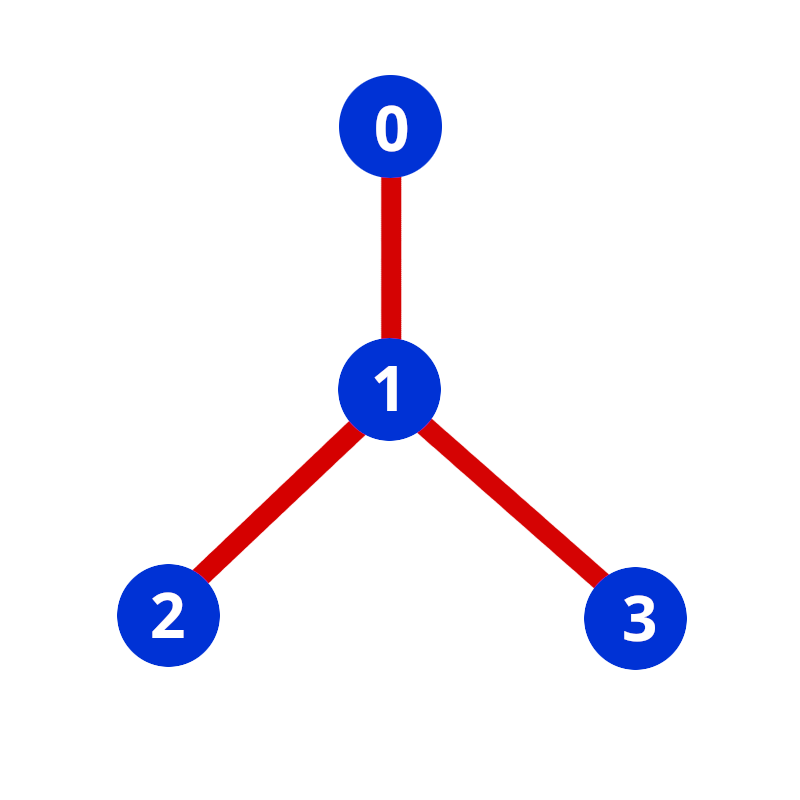
\includegraphics{../slike/topologija_simple.png}
		\end{figure}
	\end{columns}
\end{frame}

\subsection{Pobolj\v{s}anje}
\begin{frame}
\begin{columns}
	\column{0.5\textwidth}
	\begin{itemize}
		\item Brzina slanja ostala ista
		\item Kapacitet linka izme\dj{}u ra\v{c}unara 0 i 1 pove\'{c}an na 10\! Mbps
		\item O\v{c}ekujemo mali broj izgubljenih paketa
	\end{itemize}
	\column{0.5\textwidth}
	\begin{figure}
		\centering
		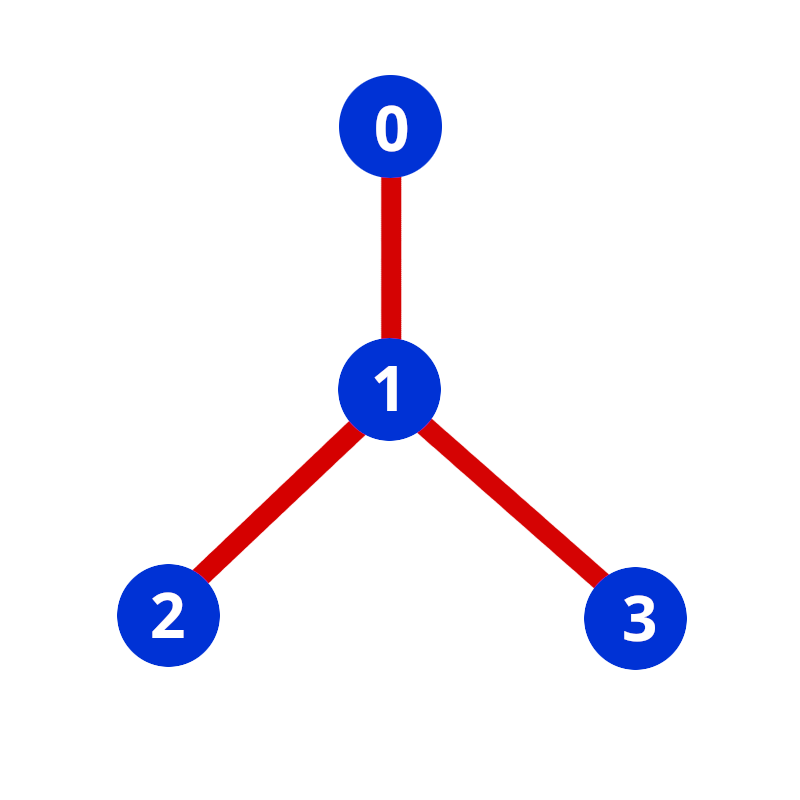
\includegraphics{../slike/topologija_simple.png}
	\end{figure}
\end{columns}
\end{frame}

\subsection{Rezultati}
\begin{frame}
	\begin{table}
		%\vspace{12pt}
		\begin{tabular}{l|rr}
			& Pre pro\v{s}irenja & Polse pro\v{s}irenja \\
			\hline
			Poslato paketa & 24998 & 24998\\
			Primljeno paketa & 13144 & 23808\\
			Izgubljeno paketa & 11854 & 1190\\
		\end{tabular}
	\end{table}
	\begin{block}{Zaklju\v{c}ak}
		\begin{itemize}
			\item Dosta manje izgubljenih paketa
			\item Procenat izgubljenih paketa smanjen sa $47.42\%$ na $4.76\%$
		\end{itemize}
	\end{block}
\end{frame}

\subsection{Napomene}
\begin{frame}
	\begin{columns}
		\column{0.5\textwidth}
		\begin{itemize}
			\item Izgubljeni paketi posle pro\v{s}irenja
			\item Izbor L4 protokola
		\end{itemize}
		\column{0.5\textwidth}
		\begin{table}[htb]
			\centering
			\begin{tabular}{l|r}
				\hline
				Poslato paketa & 12498 \\
				Primljeno paketa & 12498 \\
				Izgubljeno paketa & 0 
			\end{tabular}
		\end{table}
	\end{columns}
\end{frame}
\section{Zaklju\v{c}ak}

\begin{frame}
	\frametitle{\textit{Summa Summarum}}
	
		\begin{itemize}
			\item \v{S}ta sam o\v{c}ekivao?
			\item \v{S}ta sam postigao?
			\item Iskustva u radu sa NS-3
			\item NS-3 i PMT
		\end{itemize}
		
\end{frame}

\end{document}

